
%%% Local Variables: 
%%% mode: latex
%%% TeX-master: t
%%% End: 

\cleardoublepage

\chapter{3D播放器设计与实现}
\label{cha:3Dplayerdesignandrealization}

\section{实验平台}
\label{sec:3dplayerhardwareplatform}

%\subsection{NVIDIA 3D Vision套装介绍}
%\label{subsec:nvidia3dvisionbrief}

% 此处可以插入一段介绍以及图片

%\subsection{实验平台}
%\label{subsec:3dplayerplatform}
% 平台的介绍
我们希望利用NVIDIA 3D Vision套装进行3D播放器的立体显示。由于3D Vision只支持Windows Vista和Windows 7,所以实验的操作系统有限制。实验主要在以下环境下进行:

\begin{itemize}
\item {硬件平台}

\begin{itemize}
\item Intel Core2 Quad Q9400 @ 2.66GHz
	\footnote{SpeedStep功能关闭}
\item 4GB DDR2/800 Memory
\item NVIDIA GeForce GTS 250 with 512MB
\end{itemize}

\item {软件平台}

\begin{itemize}
\item Microsoft Windows 7 Enterprise
	\footnote{获取自:\href{http://helpdesk.tsinghua.edu.cn/yhfw/yhfw_zbrj_tz.jsp}{清华大学校园正版软件服务}}
\item NVIDIA 3D Vision Driver v1.23
\item DirectX 11.0
\item Microsoft Visual Studio 2008 SP1
	\footnote{获取自:\href{http://helpdesk.tsinghua.edu.cn/yhfw/yhfw_zbrj_tz.jsp}{清华大学校园正版软件服务}}
\end{itemize}

\end{itemize}


\section{调研阶段}
\label{sec:3Dplayersurvey}

想要实现3D播放器就需要调用硬件资源,至少要能让3D Vision的眼镜工作起来。对此,我们进行了一段时间的调研,希望找到一些资料,了解如何调用这些资源。

%nvapi

NVIDIA的3D Vision驱动盘上有一个3D播放器程序,可以用来播放NVIDIA官方网站上提供下载的一些3D视频片段。可惜这个播放器不是开源的,我们猜想其内部是利用了NVIDIA提供的API函数的,于是去NVIDIA的开发站点上下载了NVAPI\footnote{\url{http://developer.download.nvidia.com/NVAPI/NVAPI_May2009.zip}}。在NVAPI中,我们找到了和立体显示相关的部分接口函数如\autoref{lst:NVAPI}:

% 此处插入NVAPI截图
\begin{lstlisting}[caption = {NVAPI中立体显示的部分函数}, label = lst:NVAPI]
`\dots`
NVAPI_INTERFACE NvAPI_Stereo_Enable(void);
NVAPI_INTERFACE NvAPI_Stereo_Disable(void);
NVAPI_INTERFACE NvAPI_Stereo_CreateHandleFromIUnknown(IUnknown *pDevice, StereoHandle *pStereoHandle);
NVAPI_INTERFACE NvAPI_Stereo_Activate(StereoHandle stereoHandle);
NVAPI_INTERFACE NvAPI_Stereo_Deactivate(StereoHandle stereoHandle);
NVAPI_INTERFACE NvAPI_Stereo_CaptureJpegImage(StereoHandle stereoHandle, NvU32 quality);
`\dots`
\end{lstlisting}

其中的确有Stereoscopic3D子项,但是只有一些状态查询、保存当前图像等函数,并没有我们所需要的能够实现在显示图像或图形时能控制3D眼镜开启的接口。对此,我们认为是public版本的NVAPI不完整,没有包含这部分比较新的接口。我们尝试了注册NVIDIA的注册开发人员\footnote{\url{http://developer.nvidia.com/page/registered_developer_program.html}}(registered developer),期望能够获得完整版的NVAPI,但是申请一直没有得到答复。这个方向的调研到此中断。

%manual inter-view display

由于3D Vision的原理是将左右两个视点的图像交替显示,然后通过同步器控制眼镜快门使得每个时刻都只有一只眼睛能看到为其显示的图像,以此来实现双目立体显示。而在NVAPI中,我们又发现了名为NvAPI\_Stereo\_Enable()和NvAPI\_Stereo\_Activate()的两个函数,继而提出了一个问题:如果我们人工地控制程序交替显示两个视点的视频,显式地调用这两个函数(或其中之一),NVIDIA的驱动能否自动地让3D眼镜工作?

我们为此写了一个测试程序,可惜结果并不令人满意,我们看到的就是交替渲染的有重影的图像,而3D眼镜根本没有工作。

%d3d - cube demo

我们一直在NVIDIA的开发人员论坛以及各类3D相关的开发论坛上不断寻找关于3D Vision调用的尝试。尽管NVIDIA的开发人员论坛上有十几个活跃的thread是与此相关的,但是长期以来没有人回复可行的解决方案。经过一段时间的搜索,我们终于在mtbs3d.com上找到了一个帖子\footnote{\href{http://www.mtbs3d.com/phpBB/viewtopic.php?f=7&t=5072}{http://www.mtbs3d.com/phpBB/viewtopic.php?f=7\&t=5072}}声称成功地调用3D Vision显示了立体图像。有人根据该贴的说明进行了尝试表示同样获得成功,并给出了一个Demo,显示一些在屏幕上进行XYZ三个方向上平移的立方体。我们下载了该Demo程序编译运行证实可行。这个Demo是基于Direct3D的,其中没有明文调用NVIDIA的API,所以我们认为:NVIDIA的驱动对Direct3D程序能够自动启用3D眼镜。

\section{3D播放器设计}
\label{sec:3dplayerdesign}

\subsection{静态3D图像的显示}
\label{subsec:static3dimgdisp}

\begin{figure}
\begin{minipage}{0.5\textwidth}
	\centering
	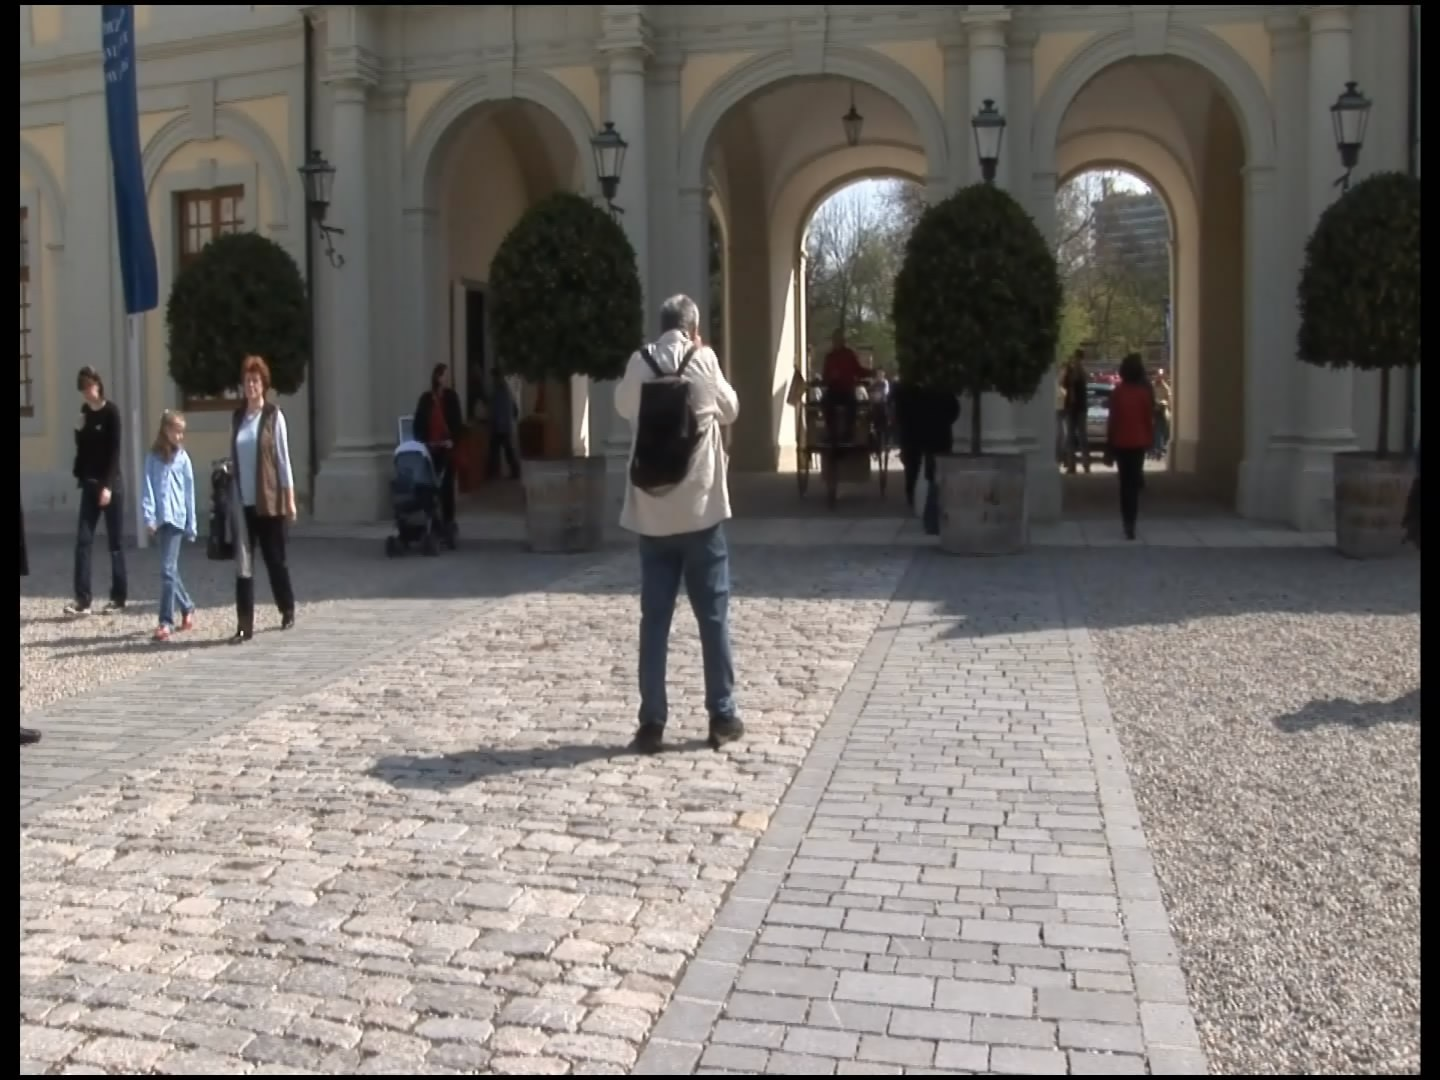
\includegraphics[width=0.95\textwidth]{staticLeftView.jpg}
	\caption{静态3D显示测试的左眼图像}
	\label{fig:staticleftview}
\end{minipage}\hfill
\begin{minipage}{0.5\textwidth}
	\centering
	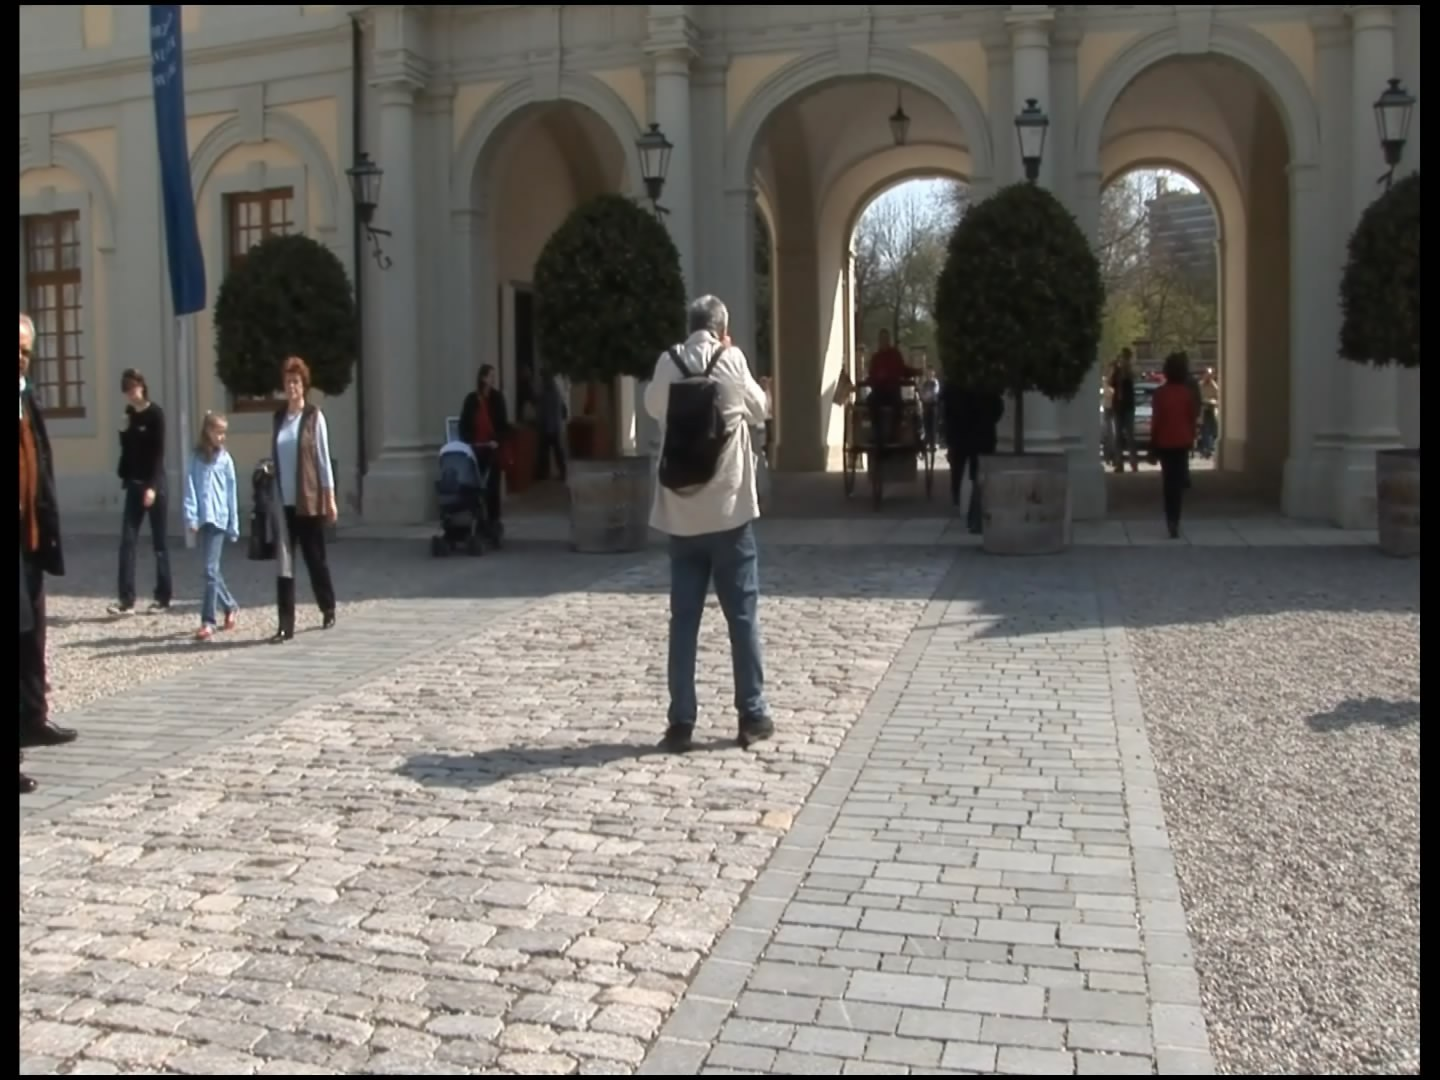
\includegraphics[width=0.95\textwidth]{staticRightView.jpg}
	\caption{静态3D显示测试的右眼图像}
	\label{fig:staticrightview}
\end{minipage}
%\caption{用于静态3D显示测试的图像}
%\label{fig:staticview}
\end{figure}

有了一次成功调用3D眼镜的经历,我们找到了一些头绪,并就此开始设计3D播放器。

我们希望3D播放器能够接收一系列的图像,这些图像分为两个序列,分别是左眼和右眼视角的图像。然后播放器以一个预设的帧率交替播放这两个序列中的图像。如果NVIDIA的驱动能够成功开启3D眼镜,此时我们通过3D眼镜就能看到立体图像了。

经过不断尝试,我们终于实现了一帧静态3D图像的显示。做法如下:

\begin{enumerate}
\item 首先我们创建一个IDirect3DSurface9,这是Direct3D中用于渲染的表面。假设我们要显示的图像的宽度和高度分别为$imgWidth$和$imgHeight$。这个表面的宽度就应该是$2\times imgWidth$,这一点较容易理解,因为有左右两个视角的图像。但是这个表面的高度必须设为$imgHeight+1$,这个多出来的1像素是上文提及的帖子中指出的关键点之一,算是一个magic number。实验中我们把高度设为$imgHeight$得到的就不是立体图,而是两幅横向并列显示的拉伸过的图像。
\item 有了这个表面之后,我们需要为其添加内容。以左上角$(0,0)$为原点,调用D3DXLoadSurfaceFromFile()读入左眼图像(\autoref{fig:staticleftview}),再以$(imgWidth,0)$为原点再次调用函数读入右眼图像(\autoref{fig:staticrightview})。
\item 在渲染之前,我们还要为这个待显示的结构写一个头,叫做$LPNVSTEREOIMAGEHEADER$,其中要指定宽度、高度、颜色深度以及一个singature,这个名为$NVSTEREO\_IMAGE\_SIGNATURE$的signature需要赋一个特定的值0x4433564e。见\autoref{lst:LPNVSTEREOIMAGEHEADER}。
\begin{lstlisting}[caption = {LPNVSTEREOIMAGEHEADER的结构}, label = lst:LPNVSTEREOIMAGEHEADER]
// Stereo Blitdefines
#define NVSTEREO_IMAGE_SIGNATURE 0x4433564e //NV3D
typedef struct _Nv_Stereo_Image_Header {
    unsigned int dwSignature;
    unsigned int dwWidth;
    unsigned int dwHeight;
    unsigned int dwBPP;
    unsigned int dwFlags;
} NVSTEREOIMAGEHEADER, *LPNVSTEREOIMAGEHEADER;
\end{lstlisting}
\item 经过如上的操作,利用Direct3D的renderer渲染输出到显示器的图像就是立体图了(\autoref{fig:staticdualview})。注意实际透过眼镜是看不到重影的,两帧图像交替显示,眼镜快门相应地轮流遮挡视线,只能看到各自视角的图像。
\end{enumerate}


\begin{figure}[htbp]
\begin{center}
\includegraphics[width=0.9\textwidth]{staticDualView.pdf}
\caption{渲染后输出的3D图像}
\label{fig:staticdualview}
\end{center}
\end{figure}

实现了一帧静态立体图的显示,就有了显示立体视频的基础,显示动态图像的部分在下一节阐述。

\subsection{立体视频(图像序列)的显示}
\label{subsec:motion3dimgdisp}

视频的显示可以看做以一个预设的帧率FPS(frames per second)显示一个图像序列中的一张张图像。这里的帧率根据视频的制式不同而改变,一般都在24或30左右。

视频中的FPS与游戏中的FPS有所不同。在游戏中,往往追求硬件所能处理的最高的FPS,尽可能使画面更加流畅。而在视频回放的时候,有一个固定的帧率,必须要尽可能让实际帧率接近这个预设的帧率,才能满足视频的每一帧出现在时间轴的正确位置上。然而,视频播放和游戏的渲染又有一个共同点,当硬件资源很有限的情况下,会将帧率降到很低,出现跳帧,这也是为了保证画面的时间正确性,避免出现像“慢动作回放”一样的效果。

综合以上的特点,我们就需要有一个控制帧率上限的机制,保证帧率在资源足够的时候不会超过预设值;同时要支持在资源受限时自动跳帧。

为了实现这样的机制,我们需要获得较为精确的时间,来控制每一帧持续的时长。ANSI C++中提供的getTicker()函数是ms级的,比较粗糙,无法满足一些常见的(如23.97)标准帧率的控制需要。对此,我们查阅了MSDN的文档后选用了Windows API中提供的QueryPerformanceCounter()和QueryPerformanceFrequency()配合实现us级的计时器。

我们实现的帧率上限控制的机制如下:在开始播放第0帧的时刻记下当前时间$t_{0}$。在渲染完第$i$帧$F_{i}$之后,获得当前时间$t_{n}$,然后准备进行第$(t_{n}-t_{0})\times FPS$的渲染。通过比较当前已渲染的帧$F_{i}$和待渲染的帧$F_{n}$是否一致来决定是否进行渲染操作。这个机制的核心就是\autoref{eqn:Fn}。
\begin{equation}\label{eqn:Fn}
F_{n}=(t_{n}-t_{0})\times FPS
\end{equation}
其中$FPS$为根据播放内容而预设的一个帧率,$t_{n}$为当前时刻,$t_{0}$为播放视频第0帧的起始时刻,$F_{n}$为当前时刻应该渲染的帧的序号。

帧率上限控制算法的伪代码见\autoref{algo:frameratecap}。

\begin{algorithm}
\caption{Frame rate cap}
\label{algo:frameratecap}
\begin{algorithmic}[1]
	\STATE $\_start \Leftarrow initialTime$ %\COMMENT{store the initial time}
	\STATE $bufferd = FALSE$
	\STATE $lastRenderedFrame \Leftarrow -1$
	\WHILE{$TRUE$}
		\STATE $\_current \Leftarrow currentTime - \_start$ %\COMMENT{get elapsed time}
		\STATE $frameToRender \Leftarrow \_current * FPS$ %\COMMENT{calc the frame to render}
		\IF{$frameToRender + 1> totalFrames$}
			\STATE $break$ \COMMENT{break when reaching the last frame}
		\ENDIF
		\IF{$buffered = FALSE$}
			\STATE load $Frame_{frameToRender+1}$ to memory
			\STATE $buffered \Leftarrow TRUE$
		\ENDIF
		\IF{$frameToRender \neq lastRenderedFrame$}
			\STATE render $Frame_{frameToRender}$
			\STATE $lastRendered \Leftarrow frameToRender$
			\STATE $buffered \Leftarrow FALSE$
		\ENDIF
	\ENDWHILE
\end{algorithmic}
\end{algorithm}

\section{播放器测试}
\label{sec:3dplayerdemo}

%功能
我们实现的播放器具有如下功能:
\begin{description}
\item[输入] 左右两个视点的图像序列文件名格式。实验中采用了“前缀+序号+后缀”的方式。前缀为文件相对路径,图像的文件名包含其对应的帧序号,后缀为文件扩展名。\\
	图像序列的总帧数$totalFrames$,见\autoref{algo:frameratecap}的第7行。\\
	播放时的帧率$FPS$,见\autoref{algo:frameratecap}的第6行。
\item[输出] 在显示器上输出如\autoref{fig:staticdualview}效果的立体图序列,帧率为$FPS$。通过3D眼镜可以看到立体视频。
\end{description}

%瓶颈

我们使用$720\times576$的分辨率对播放器进行测试,选用了几段不同的图像序列。在不断测试过程中,我们发现在图像包含告诉运动的物体时能够看出跳帧现象。于是我们输出了每一帧的load和render情况,发现实际帧率在19fps到21fps不等。我们希望寻找性能瓶颈所在,进行了以下排查:
\begin{itemize}
\item 我们首先考虑是否因为图像序列的格式为JPEG,在读取的时候需要时间解码。于是将图像序列转化为BMP格式的位图,测试发现帧率进一步降至14fps左右。测试用图存为JPEG时每帧平均大小50KB,BMP则超过300KB。
\item 有了JPEG和BMP的对比,我们认为磁盘I/O可能是一个瓶颈。对此,我们划分了500MB的内存作为一个RAMDISK。用HD Tune测试这个分区的读写速度和随机访问时间等指标如下:
\begin{description}
\item[Transfer Rate (Min)] 2751.7MB/sec
\item[Transfer Rate (Max)] 3363.2MB/sec
\item[Transfer Rate (Avg)] 3239.8MB/sec
\item[Access Time (Avg)] 0.0ms
%\item[Burst Rate] 3670.7MB/sec
%\item[CPU Usage] 0.0\%
\end{description}
将图像序列存放在该RAMDISK分区上再次进行测试,帧率依然在21fps左右。所以磁盘IO被排除在瓶颈之外。
\item 此时我们决定用性能分析工具分析我们的程序,找出其中时间耗费最多的部分,将该部分打散成多个小的函数再次分析。如此循环了几次,终于找到性能瓶颈所在:我们调用D3D中的D3DXLoadSurfaceFromFile()函数两次,分别将左右眼的图像绘制到渲染的表面上。而这两个函数调用占用了整个程序运行总时间的95\%以上。
\end{itemize}
这个API的性能我们暂时未解决,尚在寻找可行的替代方法。


\section{小结}
\label{sec:sum7}

本章介绍了3D播放器设计实现的全部过程,从调研阶段遇到的各种问题、种种尝试,到发现一种可能的解决方案,然后经过一些尝试,最终借助Direct3D实现了支持3D Vision套装的立体视频播放器。不过依然存在一定的性能瓶颈,有待进一步解决。


